\chapter{Durchführung der Analyse}
Nachdem in den vorhergegangen Abschnitten alle Aspekte des Themas "Kursanalyse von Kryptowährungen mit Azure Machine Learning" betrachtet wurden, widmet sich dieser Abschnitt der praktischen Umsetzung. Jeder Themenblock hat seinen Teil zum Erstellen eines Kontextes beigetragen, in dem die Analyse durchgeführt werden kann (siehe Tabelle \ref{tab:themeblocks}).
\begin{table}[H]
\begin{tabular}{|p{3,5cm}|p{6cm}|p{7cm}|}
\hline
\textbf{Themenblock} & \textbf{Inhalt} & \textbf{Ziel}\\ 
\hhline{===}
Data Mining Frameworks (\ref{sec:DataMiningFrameworks}) & Beschreibung der bekanntesten Frameworks des Data Mining Prozesses und Auswahl eines Frameworks für die vorliegende Arbeit & Detailliertes Beschreiben des nachfolgenden Prozessmodells\\
\hline
Machine Learning (\ref{sec:MachineLearning}) & Vorstellung einer Möglichkeit zur Einordnung von Machine Learning Typen und Algorithmen & Verständnisaufbau für die Analyse in diesem Teil der Arbeit\\
\hline
Kryptowährungen (\ref{sec:cryptocurrency2}) & Hintergrundwissen zu Kryptowährungen & Für eine Analyse ist Hintergrundwissen wichtig. Dieses sogenannte "Domain"-Wissen ist essentieller Bestandteil einer Analyse mit CRISP-DM\\
\hline
Microsoft Azure Machine Learning Studio (\ref{sec:msmls}) & Allgemeine Beschreibunng und Aufbau des Werkzeugs & Das Studio soll als Werkzeug zur Analyse eingesetzt werden.\\
\hline
\end{tabular}
\caption{Behandelte theoretische Abschnitte im Kontext der Arbeit}
\label{tab:themeblocks}
\end{table}
Wie in Punkt \ref{sec:crispdmdec} angesprochen, wird als Hilfe für das Prozessmodell CRISP-DM der zugehörige User Guide \citep[S.~30-56]{chapman_crisp-dm_2000} herangezogen. Die, im Guide genannten, Outputs jedes Prozessschritts werden nachfolgend speziell hervorgehoben. Das CRISP-DM Prozessmodell ist sehr generisch gehalten. Dies ist beispielsweise daran zu erkennen, dass das Modell in vier übereinander liegende Abstraktionsschichten gegliedert ist.\citep[S.~6]{chapman_crisp-dm_2000} Dies dient der Anpassungsfähigkeit an viele heterogene Projekte. Diese Anpassungsfähigkeit wird gleich im ersten Schritt genutzt.\newline
 
\section{Business Understanding}
\subsection{Determine the Business Objectives}
In  gewöhnlichen Industrie- oder Forschungsprojekten ist es wichtig, die Stakeholder (vor allem Geldgeber) und den Reifegrad und die Akzeptanz des Data Mining im Projektumfeld zu analysieren. Dies rückt im vorliegenden Fall in den Hintergrund. Die Anderen Outputs sind jedoch ebenso wichtig.

\begin{longtable}[H]{|p{4,5cm}|p{12cm}|}
\hline
\textbf{Output} & \textbf{Beschreibung} \\ 
\hhline{==}
Background & Die Analyse wird im Rahmen einer Masterarbeit durchgeführt. Nur eine Person ist daran beteiligt. \\
\hline
Business objectives & Die Untersuchung hat zwei Hauptziele. Das eine ist die Analyse der Cryptowährungen an sich. Es soll herausgefunden werden, ob Kursschwankungen mit Hilfe der Isolation von Einflussfaktoren und den Mitteln des Machine Learning vorausgesagt werden können oder anderweitige Auffälligkeiten zu beobachten sind. Das andere Ziel ist die Einarbeitung in das Werkzeug Azure Machine Learning. \\
\hline
Business success criteria & Die Erkenntnis, dass eine Vorhersage nicht möglich ist, oder dass wichtige Einflüsse nicht gefunden wurden, ist durchaus möglich und bedeutet keinesfalls ein Scheitern des Projekts. Hinsichtlich des Werkzeugs Azure ML, ist es beispielsweise interessant, welchen Restriktionen das Tool unterlegen ist. Das Betrifft sowohl Funktionen, die (noch) nicht vorhanden sind, oder technische Limitationen, wie Geschwindigkeit, Volumenbegrenzungen etc..\\
\hline
\caption{Output des Schrittes "Determine the Business Objectives"}
\end{longtable}

\subsection{Assess the Situation} \label{subsec:assesTheSituation}
Dieser Teil befasst sich vor allem damit, welche Ressourcen zur Verfügung stehen (Hardware, Software, personell) und welche sonstigen Bedingungen erfüllt sein müssen oder das Projekt begrenzen. Dazu zählt auch das Finden von Daten, die für die Modellierung genutzt werden können. Anzumerken ist hierbei, dass es noch nicht um das tatsächliche Laden der Daten im Sinne von Dateien geht, sondern um das Finden von potentiellen Quellen für Daten. Zusätzlich sollen noch eine Risiko- und eine Kosten-Nutzen-Analyse durchgeführt werden. Das Hauptaugenmerk liegt jedoch auf der Erschließung der Daten. 
\newline
An Stelle einer vollständigen Risikoanalyse (Kontext herstellen, Risiken identifizieren, analysieren, evaluieren, managen\citep[S.~43]{sowa_management_2017}), tritt eine Aufzählung der 3 Hauptrisiken. Dies geschieht einerseits aus Gründen der Verhältnismäßigkeit, andererseits liegt der Fokus der Arbeit auf einem anderen Thema. Ähnlich verhält es sich mit der Kosten-Nutzen-Analyse. Sie wird zur Bewertung der Wirtschaftlichkeit herangezogen, was in diesem Kontext nicht relevant ist. Deswegen wird auf sie vollständig verzichtet.
\newline
Die schwerste Aufgabe dieses Teils ist das Finden von Daten, die Einfluss auf den Kurs von Kryptowährungen haben (könnten). Forschungen in diesem Bereich identifizierten einerseits öffentliches Interesse (soziale Medien, Google Suchanfragen, etc.)\multicitep{kristoufek_bitcoin_2013; garcia_digital_2014} und andererseits auch wirtschaftliche Faktoren ("standard economic theory", also Angebot und Nachfrage, Investoren)\citep{kristoufek_what_2015} als Haupteinflussfaktoren. Anhand den Aussagen dieser Paper und zusätzlichen Überlegungen ergeben sich folgende Faktoren, die bei der Analyse bedacht werden (Tabelle \ref{tab:dataToAnalyse}).\newline Darüber hinaus wird die Quelle aufgeführt, über die die Daten bezogen werden. Bei monetären Strömen oder Kursen, wird immer der Kurs in USD herangezogen. 
\newline
Damit eine Analyse der Kryptowährungen möglich ist, müssen zu diesen historische Kursdaten beschafft werden. Dieser, auf den ersten Blick simpel wirkende Schritt, ist in Wirklichkeit \todo{formulierung} nicht trivial. Kryptowährungen werden an dutzenden Portalen gleichzeitig gehandelt. Dabei erscheinen genauso schnell neue Börsen, wie alte verschwinden. Auch das Handelsvolumen und die Handelswährung unterscheidet sich. Hinzu kommt, dass an Bitcoin- oder Ethereum-Handelsportalen meist 24 Stunden täglich gehandelt werden kann. Aus diesem Grund sind solche Datenquellen ausgewählt worden, die entweder ihre Daten direkt von der Blockchain erhalten oder einen gewichteten Mittelwert über die größten Handelsplatformen berechnen.
\newline
Die nächste Schwierigkeit ist die Auswahl der Aktienindizes, die für die Analyse herangezogen werden. Es existiert keine allgemein gültige oder anerkannte Liste mit 'den wichtigsten Aktienindizes'. Aus diesem Grund wurden die Indices ausgewählt, die die Website investing.com als "major world indices" deklariert.\citep{fusion_media_limited_major_2017} Es liegt dabei eine große Überschneidung mir anderen Stock Market-Seiten vor.\multicitep{liveindex.org_live_2017; yahoo_finance_major_2017; yahoo_finance_major_2017-1} Zusätzlich zu den Aktienindices wird ein Financial Stress Index (FSI) herangezogen. Ein solcher "index misst die aktuelle Belastung in einem finanzwirtschaftlichen System"\citep[S.~1;eigene Übersetzung]{vermeulen_financial_2014} In diesem Fall ist es der St. Louis Fed Financial Stress Index, der 18 Einzelfaktoren aus drei Kategorien bündelt.\citep{federal_reserve_bank_of_st._louis_st._2017}
\newline
Ferner werden die Währungen der acht größten Volkswirtschaften\citep{the_international_monetary_fund_world_2017} und die Kurse für Gold, Silber und Rohöl mit einbezogen. Es werden die Wechselkurse zum Dollar betrachtet, sprich Fremdwährung/USD. Bei den Ölkursen wird Brent, das wichtigste Rohöl für den europäischen Markt \citep{noauthor_brent_2016}, und West Texas Intermediate (WTI), das Pondon für den US-Markt, betrachtet\citep{noauthor_west_2017}.

\begin{longtable}[H]{|p{4cm}|p{6,25cm}|p{6,25cm}|}
\multicolumn{3}{c}{\textit{Cryptowährungs-eigene Faktoren}}\\ \hline
\textbf{Daten} & \textbf{für BTC} & \textbf{für ETH} \\
\hhline{===}
Handelsvolumen & ja, von https://bitcoincharts.com/ &  ja, von https://coinmarketcap.com/ \\ \hline
Coin Volumen (Gesamtanzhal der vorhandenen Bitcoins/des Ethers) & ja, von https://blockchain.info/ & ja, von https://etherscan.io/ \\ \hline
Mining-Schwierigkeit \todo{Erklärung} & ja, von https://data.bitcoinity.org/ & ja, von https://etherscan.io/ \\ \hline
Anzahl der Transaktionen & ja, von https://blockchain.info/ & ja, von https://etherscan.io/ \\ \hline
Hashrate & ja, von https://www.kaggle.com/ & ja, von https://www.kaggle.com/ \\ \hline
Marktkapitalisierung & ja, von https://www.kaggle.com/ & ja, von https://www.kaggle.com/ \\ \hline
\multicolumn{3}{c}{\textit{Öffentliches Interesse}}\\ \hline
\textbf{Daten} & \textbf{für BTC} & \textbf{für ETH} \\
\hhline{===}
Google Websuchen & ja, von https://trends.google.de/trends/ & ja, von https://trends.google.de/trends/ \\ \hline
Google News-Suchen & ja, von https://trends.google.de/trends/ & ja, von https://trends.google.de/trends/ \\ \hline
Wikipedia Seitenaufrufe & ja, von https://wikimedia.org/api/rest \textunderscore v1/ & ja, von https://wikimedia.org/api/rest \textunderscore v1/ \\ \hline
Tweets (Twitter Nachrichten) & \multicolumn{2}{c}{nein, nicht kostenlos verfügbar} \\ \hline
Zeitungsartikel/-Überschriften & \multicolumn{2}{c}{ja, von https://www.kaggle.com/therohk/million-headlines/data/}\\ \hline
Blogartikel & \todo{???} & \todo{???} \\ \hline
(Web-)Domains & \todo{???} & \todo{???} \\ \hline
\multicolumn{3}{c}{\textit{(Aktien)indizes}}\\ \hline
\textbf{Daten} & \textbf{für BTC} & \textbf{für ETH} \\
\hhline{===}
Dow 30	& \multicolumn{2}{c}{ja, von https://www.investing.com/indices/}\\ \hline
S\&P 500	& \multicolumn{2}{c}{ja, von https://www.investing.com/indices/}\\ \hline
Nasdaq	 & \multicolumn{2}{c}{ja, von https://www.investing.com/indices/}\\ \hline
SmallCap & \multicolumn{2}{c}{ja, von https://www.investing.com/indices/}\\ \hline
S\&P 500 VIX& \multicolumn{2}{c}{ja, von https://www.investing.com/indices/}\\ \hline
S\&P/TSX	& \multicolumn{2}{c}{ja, von https://www.investing.com/indices/}\\ \hline
TR Canada  & \multicolumn{2}{c}{ja, von https://www.investing.com/indices/}\\ \hline
Bovespa	& \multicolumn{2}{c}{ja, von https://www.investing.com/indices/}\\ \hline
IPC & \multicolumn{2}{c}{ja, von https://www.investing.com/indices/}\\ \hline
DAX	& \multicolumn{2}{c}{ja, von https://www.investing.com/indices/}\\ \hline
FTSE 100		& \multicolumn{2}{c}{ja, von https://www.investing.com/indices/}\\ \hline
CAC 40	 	& \multicolumn{2}{c}{ja, von https://www.investing.com/indices/}\\ \hline
Euro Stoxx 	& \multicolumn{2}{c}{ja, von https://www.investing.com/indices/}\\ \hline
AEX		& \multicolumn{2}{c}{ja, von https://www.investing.com/indices/}\\ \hline
IBEX 	& \multicolumn{2}{c}{ja, von https://www.investing.com/indices/}\\ \hline
FTSE MIB	& \multicolumn{2}{c}{ja, von https://www.investing.com/indices/}\\ \hline	
SMI		& \multicolumn{2}{c}{ja, von https://www.investing.com/indices/}\\ \hline
PSI 	& \multicolumn{2}{c}{ja, von https://www.investing.com/indices/}\\ \hline
BEL 	& \multicolumn{2}{c}{ja, von https://www.investing.com/indices/}\\ \hline	 
ATX		& \multicolumn{2}{c}{ja, von https://www.investing.com/indices/}\\ \hline
OMXS30		& \multicolumn{2}{c}{ja, von https://www.investing.com/indices/}\\ \hline
OMXC20	& \multicolumn{2}{c}{ja, von https://www.investing.com/indices/}\\ \hline	
MICEX		& \multicolumn{2}{c}{ja, von https://www.investing.com/indices/}\\ \hline
RTSI	& \multicolumn{2}{c}{ja, von https://www.investing.com/indices/}\\ \hline	
WIG20		& \multicolumn{2}{c}{ja, von https://www.investing.com/indices/}\\ \hline
Budapest SE		& \multicolumn{2}{c}{ja, von https://www.investing.com/indices/}\\ \hline
BIST 100	& \multicolumn{2}{c}{ja, von https://www.investing.com/indices/}\\ \hline	
TA 35		& \multicolumn{2}{c}{ja, von https://www.investing.com/indices/}\\ \hline	 
Tadawul All Share	& \multicolumn{2}{c}{ja, von https://www.investing.com/indices/}\\ \hline
Nikkei 225		& \multicolumn{2}{c}{ja, von https://www.investing.com/indices/}\\ \hline
S\&P/ASX 200		& \multicolumn{2}{c}{ja, von https://www.investing.com/indices/}\\ \hline
DJ New Zealand		& \multicolumn{2}{c}{ja, von https://www.investing.com/indices/}\\ \hline
Shanghai	& \multicolumn{2}{c}{ja, von https://www.investing.com/indices/}\\ \hline
SZSE Component		& \multicolumn{2}{c}{ja, von https://www.investing.com/indices/}\\ \hline
China A50		& \multicolumn{2}{c}{ja, von https://www.investing.com/indices/}\\ \hline
DJ Shanghai	& \multicolumn{2}{c}{ja, von https://www.investing.com/indices/}\\ \hline
Hang Seng		& \multicolumn{2}{c}{ja, von https://www.investing.com/indices/}\\ \hline
Taiwan Weighted		& \multicolumn{2}{c}{ja, von https://www.investing.com/indices/}\\ \hline
SET		& \multicolumn{2}{c}{ja, von https://www.investing.com/indices/}\\ \hline
KOSPI	& \multicolumn{2}{c}{ja, von https://www.investing.com/indices/}\\ \hline
IDX Composite	& \multicolumn{2}{c}{ja, von https://www.investing.com/indices/}\\ \hline
Nifty 	& \multicolumn{2}{c}{ja, von https://www.investing.com/indices/}\\ \hline
BSE Sensex	& \multicolumn{2}{c}{ja, von https://www.investing.com/indices/}\\ \hline
PSEi Composite	& \multicolumn{2}{c}{ja, von https://www.investing.com/indices/}\\ \hline
STI Index	& \multicolumn{2}{c}{ja, von https://www.investing.com/indices/}\\ \hline
Karachi	& \multicolumn{2}{c}{ja, von https://www.investing.com/indices/}\\ \hline
HNX 30	& \multicolumn{2}{c}{ja, von https://www.investing.com/indices/}\\ \hline
CSE All-Share	& \multicolumn{2}{c}{ja, von https://www.investing.com/indices/}\\ \hline


St. Louis Fed Financial Stress Index (STLFSI) & \multicolumn{2}{c}{ja, von https://fred.stlouisfed.org/series/STLFSI}\\ \hline
\multicolumn{3}{c}{\textit{Währungen der größten Volkswirtschaften (nach BIP)}}\\ \hline
\textbf{Daten} & \textbf{für BTC} & \textbf{für ETH} \\
\hhline{===}
China (CNY) & \multicolumn{2}{c}{ja, von https://www.investing.com/currencies/single-currency-crosses}\\ \hline
Japan (JPY)& \multicolumn{2}{c}{ja, von https://www.investing.com/currencies/single-currency-crosses}\\ \hline
Deutschland (EUR) & \multicolumn{2}{c}{ja, von https://www.investing.com/currencies/single-currency-crosses}\\ \hline
Großbritannien  (GBP) & \multicolumn{2}{c}{ja, von https://www.investing.com/currencies/single-currency-crosses}\\ \hline
Frankreich (EUR) & \multicolumn{2}{c}{ja, von https://www.investing.com/currencies/single-currency-crosses}\\ \hline
Indien (INR) & \multicolumn{2}{c}{ja, von https://www.investing.com/currencies/single-currency-crosses}\\ \hline
Brasilien (BRL) & \multicolumn{2}{c}{ja, von https://www.investing.com/currencies/single-currency-crosses}\\ \hline
\multicolumn{3}{c}{\textit{natürliche Ressourcen}}\\ \hline
\textbf{Daten} & \textbf{für BTC} & \textbf{für ETH} \\
\hhline{===}
Goldpreis & \multicolumn{2}{c}{ja, von https://www.investing.com/commodities/}\\ \hline
Silberpreis & \multicolumn{2}{c}{ja, von https://www.investing.com/commodities/}\\ \hline
Brent (Rohöl Europa) & \multicolumn{2}{c}{ja, von https://www.investing.com/commodities/}\\ \hline
WTI (Rohöl USA) & \multicolumn{2}{c}{ja, von https://www.investing.com/commodities/}\\ \hline
\caption{Mögliche Einflussfaktoren auf den Kurs von Kryptowährungen}
\label{tab:dataToAnalyse}
\end{longtable}

\begin{longtable}[H]{|p{6,5cm}|p{10cm}|}
\hline
\textbf{Output} & \textbf{Beschreibung} \\ 
\hhline{==}
Inventory of resources & Personal
\begin{itemize}
\item 1 Person mit Zugang zu den Recherche Ressourcen der Hochschule München (OPAC, DBIS, ZDB etc.\citep{noauthor_hochschule_2017})
\end{itemize}
Hardware
\begin{itemize}
\item 1 PC (CPU: AMD Ryzen 5 1600 Sechskern; RAM: 8GB; GPU: NVIDIA GeForce GTX 1060 (6GB VRAM); Windows 10 Education Build 15063.674)
\end{itemize}
Software
\begin{itemize}
\item 1 "Free"-Account Microsoft Azure Machine Learning Studio mit Workspace in "South Central US"
\item Version des Juypter Notebooks 5.1.0
\item Auf dem PC: R Version 3.4.1
\item Auf dem PC: RStudio Version 1.0.153
\item Excel 2016 (Microsoft Office 365 ProPlus) Version 1710
\item Notepad++ Version 7.5.1
\end{itemize}
Daten
\begin{itemize}
\item in Tabelle \ref{tab:dataToAnalyse} genannte Daten
\item Kurse BTC/USD und ETH/USD
\item Zusätzliche Eigenschaften von Bitcoin und Ethereum. \citep{srk_cryptocurrency_2017} stellt unter der 'CC0: Public Domain'-Lizenz einen Datensatz zur Verfügung, der besondere Eigenschaften der Währungen enthält. Beispiele für Bitcoin sind die "Anzahl der einzigartigen Adressen" in der "Bitcoin Blockchain"; oder die "Anzahl der uncles pro Tag"\citep[eigene Übersetzung]{srk_cryptocurrency_2017} für Ethereum.
\end{itemize}
\\
\hline
Requirements, assumptions, and constraints & Zu Bedenken ist, dass bei einer kostenlosen Subscription im Azure ML Studio nur 10GB Storage verfügbar sind. Zusätzlich müssen Daten, die analysiert werden sollen, in das Tool geladen werden. Bei einem Upload vom PC wird das durch die Upload-Bandbreite limitiert. Eventuell müssen Daten im Projektverlauf auch öfter Hochgeladen werden, was zu Verzögerungen führen könnte. Außerdem lässt sich in der freien Version nur jeweils ein Experiment gleichzeitig ausführen. Das parallele Trainieren von Modellen ist somit nicht möglich.\newline 
Obwohl zur Hilfe neben der Web-IDE auch RStudio genutzt werden kann, soll die Untersuchung hauptsächlich mit den Azure ML Studio Bordmitteln durchgeführt werden. \newline
Schließlich sollen nur solche Daten genutzt werden, die entweder frei verfügbar sind oder mit dem Hochschulzugang zu beschaffen sind. Das schließt präparierte Datensätze von Bezahlseiten aus.\\
\hline
Risks and contingencies & \begin{itemize}
\item keinen Zugriff auf Azure ML Studio (Server-seitige Probleme; Ablauf der Free-Subscription)
\item benötigte Daten nicht verfügbar
\item \todo{todo}
\item\todo{todo}
\end{itemize} \\
\hline
Terminology & Als Glossar dient das Abkürzungsverzeichnis zu Beginn der Arbeit. \\
\hline
Costs and benefits & --- \\
\hline
\caption{Output des Schrittes "Assess the Situation"}
\end{longtable}


\subsection{Determine the Data Mining Goals}


\begin{longtable}[!h]{|p{4,5cm}|p{12cm}|}
\hline
\textbf{Output} & \textbf{Beschreibung} \\ 
\hhline{==}
Data mining goals & Es sollen mit Hilfe von Azure Machine Learning Studio mehrere Machine Learning Models erzeugt werden. Sie sollen folgende Sachverhalte \todo{Wort} vorhersagen:
\begin{itemize}
\item Steigt der Kurs innerhalb eines 24-Stunden Zyklus über das Hoch des vorhergehenden 24-Stunden Zyklus? (Mögliche Antworten sind $ja := 1$ und $nein := 0$) 
\item Fällt der Kurs innerhalb eines 24-Stunden Zyklus unter das Tief des vorhergehenden 24-Stunden Zyklus? (Mögliche Antworten sind $ja := 1$ und $nein := 0$)
\item Wie hoch ist das Hoch des nächsten 24-Stunden Zyklus? (Antwort: Preis eines Bitcoins/Ethers in USD)
\item Wie niedrig ist das Tief des nächsten 24-Stunden Zyklus? (Antwort: Preis eines Bitcoins/Ethers in USD)
\end{itemize} 
Bei den ersten beiden Fällen handelt es sich um eine two-class classification (siehe \ref{subsubsec:classification}). Die letzten beiden Fragen fallen in das Gebiet der Regressionen (siehe \ref{subsubsec:regression}). \\
\hline
Data mining success criteria & Die Klassifikationen werden bewertet anhand:
\begin{itemize}
\item Accuracy: $ \frac{t_{p} + t_{n}}{t_{p} + t_{n} + f_{p} + f_{n}}$ (Anteil der insgesamt richtig vorhergesagten Werte)
\item Precision: $ \frac{t_{p}}{t_{p} + f_{p}}$ (Anteil der richtig vorhergesagten true-Werte)
\item Recall: $ \frac{t_{p}}{t_{p} + f_{n}}$ (Anteil der richtig vorhergesagten true-Werte an allen eigentlich richtigen true-Werten)
\item F1-score: $ 2 \times \frac{Precision \times Recall}{Precision + Recall}$ (Harmonisches Mittel aus Precision und Recall; Bester Wert = 1)
\item AUC: Fläche unter der Receiver Operating Characteristics (ROC) Kurve; "Je besser die Klassifizierungsfähigkeit des Klassifikators desto höher ist der AUC-Wert"\citep[ROC-Kurve]{lohninger_grundlagen_2013} 
\end{itemize} 
$ t_{p} : true \quad positive $ \newline
$ t_{n} : true \quad negative $ \newline
$ f_{p} : false \quad positive $ \newline
$ f_{n} : false \quad negative $ \newline
\\
& Die Regressionen werden bewertet anhand:
\begin{itemize}
\item Mean absolute error (MAE): Unterschied von vorhergesagten und tatsächlichen Werten; je kleiner desto besser\citep{mircosoft_evaluate_2017}
\item Root mean squared error (RMSE): Macht eine Aussage darüber, "wie gut eine Funktionskurve an vorliegende Daten angepasst ist"; "je größer der RMSE [...], desto schlechter"\citep{statista_root_nodate}
\item Relative absolute error (RAE), Relative squared error (RSE): Ähnlich dem RMSE, aber für den Vergleich von Regressionen mit unterschiedlichen Maßeinheiten geeignet.\citep{dr._sayad_model_2017} Im vorliegenden Fall können die anderen Größen herangezogen werden, da alle Modelle die gleiche Einheit für die vorhergesagten Werte nutzen.
\item Coefficient of determination: Gütemaß für die Aussagekraft der Regression; 
\newline
$Regression \quad passt \quad perfekt := 1$ 
\newline 
$Regression \quad erklärt \quad nichts := 0$;
\newline 
kleine Werte sind normal, große  sollten misstrauisch machen\citep{mircosoft_evaluate_2017}
\end{itemize}
\\
\hline
\caption{Output des Schrittes "Determine the Data Mining Goals"}
\end{longtable}


\todo{welche werte bedeuten was} \newline
\todo{bessere beschreibungen} \newline
\todo{was zu den quellen sagen}

\subsection{Produce a Project Plan}
Nach diesem sehr Daten-orientierten Teilschritt, befasst sich der nachfolgende Schritt einerseits mit der (groben) Planung des weiteren Projekts und andererseits mit einer anfänglichen Betrachtung der eingesetzten Werkzeuge. Grundsätzlich orientiert sich der Projektplan am Referenzmodell CRISP-DM. In einem komplexeren Projekt mit mehreren kollaborativ arbeitenden Personen, kommt diesem Schritt eine größere Rolle zu als im vorliegenden Fall. Wichtige Meilensteine, die zu bestimmten Zeitpunkten fertig vorliegen müssen, um einen unterbrechungsfreien Projektverlauf zu gewährleisten, stellen die Outputs jedes Prozessschrittes dar. Eine genauere zeitliche Einschätzung ist dem Output "Project Plan" in Tabelle \ref{tab:projectPlan} zu entnehmen. Zu sehen ist dort, die geschätzte Arbeitszeit in Tagen für jeden Schritt und der Anteil am Gesamtprojekt. Anzumerken ist hier, dass die Angaben durch Rückschritte in frühere Phasen verzerrt werden können.\newline
Bei der initialen Betrachtung der Werkzeuge werden laut Prozessmodell verschiedene alternativen gegeneinander abgewogen und ihr Zweck im Projekt festgelegt. Da das Werkzeug Azure Machine Learning Studio bereits vorgegeben ist, wird hier nur der Zweck der Werkzeuge im Projektverlauf betrachtet. Wird das Werkzeug R (bzw. RStudio) eingesetzt, so erhält es den Vorzug gegenüber seiner Konkurrenz (z.b. Python) aufgrund der Erfahrung des Entwicklers.


\begin{longtable}[!h]{|p{4cm}|p{4cm}|p{4cm}|}
\hline
\textbf{Prozessschritt} & \textbf{geschätze Zeit in Tagen} & \textbf{Prozentualer Anteil} \\
\hhline{===}
Collect initial data & 2 & 20\% \\ \hline
Describe data & 2 & 20\% \\ \hline
Explore data & 2 & 20\% \\ \hline
Verify data quality & 2 & 20\% \\ \hline
Data understanding gesamt & $\sum 2$ &  $\sum 2 \%$ \\ \hline
Select data & 2 & 20\% \\ \hline
Clean data & 2 & 20\% \\ \hline
Construct data & 2 & 20\% \\ \hline
Integrate data & 2 & 20\% \\ \hline
Format data  & 2 & 20\% \\ \hline
Data preparation gesamt & $\sum 2$ &  $\sum 2 \%$ \\ \hline
Select modeling technique & 2 & 20\% \\ \hline
Generate test design & 2 & 20\% \\ \hline
Build model & 2 & 20\% \\ \hline
Assess model & 2 & 20\% \\ \hline
Modeling gesamt & $\sum 2$ &  $\sum 2 \%$ \\ \hline
Evaluate results & 2 & 20\% \\ \hline
Review process & 2 & 20\% \\ \hline
Determine next steps & 2 & 20\% \\ \hline
Evaluation gesamt & $\sum 2$ &  $\sum 2 \%$ \\ \hline
Plan deployment & 2 & 20\% \\ \hline
Plan monitoring and maintenance & 2 & 20\% \\ \hline
Produce final report & 2 & 20\% \\ \hline
Review project & 2 & 20\% \\ \hline
\caption{Output "Project Plan" des Schrittes "Produce a Project Plan"}
\label{tab:projectPlan}
\end{longtable}

\begin{longtable}[!h]{|p{4cm}|p{11cm}|}
\hline
\textbf{Werkzeug} & \textbf{Zweck im Projekt}\\ 
\hhline{==}
Microsoft Azure Machine Learning Studio & Vorgabe im Projekt; soll in jeder Phase genutzt werden, wo es möglich ist \\ \hline
Juypter Notebooks & Integriert in Azure ML Studio; für R Code, der in der Cloud ausgeführt werden soll \\ \hline
R & zur Nutzung in Situationen für die Azure ML keine vorgefertigten Experiment Items bereitstellt \\ \hline
RStudio & zum lokalen entwerfen von Scripten vor der Ausführung in der Cloud und zur Vorbereitung der Datensätze \\ \hline
Excel & zur Betrachtung, Vorbereitung und Konvertierung von Daten vor dem Upload in die Cloud \\ \hline
Notepad++ & zur Betrachtung, Vorbereitung und Konvertierung von Daten vor dem Upload in die Cloud \\ \hline
\caption{Output "Initial assessment of tools and techniques" des Schrittes "Produce a Project Plan"}
\label{tab:projectPlan}
\end{longtable}


\section{Data Understanding}
\subsection{Collect the Initial Data} \label{subsec:collection}
In Schritt \ref{subsec:assesTheSituation} wurden Einflussfaktoren auf den Kurs festgehalten. Zusätzlich wurden bereits Quellen für Daten zu diesen Faktoren gesucht. In diesem Schritt werden nun die Daten tatsächlich (im Sinne von 'echten' Dateien) bezogen und bereits in Azure Machine Learning geladen. Ebenfalls Teil dieses Schrittes ist es, die Daten grob zu beschreiben. Im vorliegen Fall wird die Datenspanne und weitere offensichtliche Merkmale beschrieben. \newline

Die Herkunft der Daten ist nicht weiter beschrieben, da dies bereits in \ref{subsec:assesTheSituation} abgehandelt wurde. \newline

Alle gesammelten Daten enthalten Header-Informationen (Preis, Kurs, Datum etc.). Azure ML Studio kann diese Header auslesen und nutzt sie für einfache Select- oder Join-Befehle. Damit dies möglich ist, müssen die Daten als 'Genereic CSV File with a header (.csv)' oder 'Generic TSV File with a header (.tsv)' vorliegen. In manchen Fällen ist es möglich, dass Microsoft Excel beim Speichern einer Datei als '.csv' statt Kommas, Strichpunkte zum Trennen nutzt. Hier ist darauf zu achten, dass tatsächlich Kommas als Trennzeichen genutzt werden, da Azure ML Studio diese sonst nicht interpretieren kann. Die Datei-Endung '.tsv' ist nicht zwingend erforderlich. Ein 'Tab seperated values'-File kann auch mit der Endung '.txt' hochgeladen und richtig interpretiert werden. Dies ist wichtig, da Excel als Endung für diese Dateien nicht '.tsv' sondern '.txt' wählt.\newline

Azure ML Studio bietet die Möglichkeit, mehrere Dateien gezippt in das Tool zu laden. Dies bietet sich an, wenn viele einzelne Dateien hochgeladen werden sollen. Leider kann das Zip-File pro Experiment nur einmal verwendet werden und nur eine Datei daraus kann entpackt werden. Dadurch ist diese Option im Falle dieser Arbeit nicht praktikabel. Es müssen also alle Dateien einzeln geladen werden.

\begin{longtable}[!h]{|p{5cm}|p{4cm}|p{5cm}|}
\hline
\multicolumn{3}{|c|}{Cryptowährungs-eigene Faktoren}\\ \hline
\textbf{Datensatz} & \textbf{Reichweite} & \textbf{Besonderheiten}\\ 
\hhline{===}
BTC \textunderscore Total \textunderscore Volume \textunderscore Daily \textunderscore Full & 3.1.2009 bis 5.11.2017 & teilweise kein Anstieg des Volumens im Datensatz; große Lücken im Datensatz (2012-2016)\\ \hline
BTC \textunderscore Difficulty \textunderscore Daily \textunderscore Full & 6.11.2012 bis 5.11.2017 & Zeit in UTC \\ \hline
BTC \textunderscore Transaction \textunderscore Number \textunderscore Fully \textunderscore Daily & 3.1.2009 bis 5.11.2017 & \\ \hline
BTC \textunderscore Price \textunderscore Multiple \textunderscore Daily & 17.7.2010 bis 5.11.2017 & Zeit in UTC; sehr Lückenhaft, da erst ab 2016 alle enthaltenen Börsen operieren \\ \hline
ETH \textunderscore Total \textunderscore Volume \textunderscore Daily \textunderscore Full & 30.7.2015 bis 5.11.2017 & Zeit in UTC und UnixTimeStamp \\ \hline
ETH \textunderscore Difficuly \textunderscore Daily \textunderscore Full & 30.7.2015 bis 5.11.2017 & Zeit in UTC und UnixTimeStamp \\ \hline
ETH \textunderscore Transaction \textunderscore Number \textunderscore Fully \textunderscore Daily &  30.7.2015 bis 5.11.2017 & Zeit in UTC und UnixTimeStamp; ganz am Anfang einige 0-Werte \\ \hhline{===}

\multicolumn{3}{|c|}{Öffentliches Interesse}\\ \hline
\textbf{Datensatz} & \textbf{Reichweite} & \textbf{Besonderheiten}\\ 
\hhline{===}
google \textunderscore Trends \textunderscore BTC \textunderscore Websearch & 01.2009 bis 11.2017 & Daten im Abstand von 1 Monat; auf einer Scala von 0-100; erster nicht-null-Wert bei 05.2011 \\ \hline
google \textunderscore Trends \textunderscore ETH \textunderscore Websearch & 01.2011 bis 11.2017 & Daten im Abstand von 1 Monat; auf einer Scala von 0-100; erster nicht-null-Wert bei 08.2014 \\ \hline
google \textunderscore Trends \textunderscore BTC \textunderscore Newssearch & 01.2009 bis 11.2017 & Daten im Abstand von 1 Monat; auf einer Scala von 0-100; erster nicht-null-Wert bei 04.2011 \\ \hline
google \textunderscore Trends \textunderscore ETH \textunderscore Newssearch & 01.2011 bis 11.2017 & Daten im Abstand von 1 Monat; auf einer Scala von 0-100; erster nicht-null-Wert bei 07.2014 \\ \hline
Wiki \textunderscore Page \textunderscore Views \textunderscore BTC & 1.7.2015 bis 7.11.2017 & Enthält Datum als zusammengesetzte Zahl im Format yyyyddmm00; enthält 7 Features, von denen 5 für jede Zeile gleich sind \\ \hline
Wiki \textunderscore Page \textunderscore Views \textunderscore ETH & 1.7.2015 bis 7.11.2017 & Enthält Datum als zusammengesetzte Zahl im Format yyyyddmm00; enthält 7 Features, von denen 5 für jede Zeile gleich sind \\ \hline
abcnews \textunderscore Date \textunderscore Text & 19.2.2003 bis 30.9.2017 & großer Datensatz; viel Text; kann von Excel nicht komplett geöffnet werden \\ \hhline{===}

\multicolumn{3}{|c|}{(Aktien)indizes}\\ \hline
\textbf{Datensatz} & \textbf{Reichweite} & \textbf{Besonderheiten}\\ 
\hhline{===}
AEX, BFX, XU100, BVSP, VIX, CSE, GDAXI, DJI, FTSE, FTMIB, HSI, IBEX, MXX, JKSE, KSE, KS11, MCX, IXIC, NSEI, N225, OMXC20, OMXS30, IRTS, SPX, AXJO, GSPTSE, SSEC, SSMI, TA35, TASI, TRX50CAP, US2000, WIG20 & 1.1.2009 bis 9.11.2017 & alle Indices enthalten Lücken für Wochenenden und Feiertage; Datum in einem Format mit Text (!); gilt auch für nachfolgende Datensätze mit anderen Zeitspannen \\ \hline
ATX (ATX) \textunderscore history.txt & 23.3.2015 bis 9.11.2017 & verhältnismäßig kurze Zeitspanne \\ \hline
BSE Sensex 30 (BSESN) \textunderscore history.txt & 24.2.2011 bis 9.11.2017 & \\ \hline
Budapest SE (BUX) \textunderscore history.txt & 7.3.2011 bis 9.11.2017 & \\ \hline
Dow Jones New Zealand (NZDOW) \textunderscore history.txt & 25.8.2011 bis 9.11.2017 & \\ \hline
Dow Jones Shanghai (DJSH) \textunderscore history.txt & 6.3.2011 bis 9.11.2017 & \\ \hline
Euro Stoxx 50 (STOXX50E) \textunderscore history.txt & 15.8.2011 bis 9.11.2017 & \\ \hline
FTSE China A50 (FTXIN9) \textunderscore history.txt & 19.3.2010 bis 9.11.2017 & \\ \hline
FTSE Straits Times Singapore (STI) \textunderscore history.txt  & 7.3.2011 bis 9.11.2017 & \\ \hline
HNX 30 (HNX30) \textunderscore history.txt & 4.11.2014 bis 9.11.2017 & verhältnismäßig kurze Zeitspanne \\ \hline
PSEi Composite (PSI) \textunderscore history.txt & 3.11.2011 bis 9.11.2017 & \\ \hline
PSI 20 (PSI20) \textunderscore history.txt & 25.4.2010 bis 9.11.2017 & \\ \hline
SET Index (SETI) \textunderscore history.txt & 18.3.2011 bis 9.11.2017 & \\ \hline
SZSE Component (SZSC1) \textunderscore history.txt & 14.9.2012 bis 9.11.2017 & \\ \hline
Taiwan Weighted (TWII) \textunderscore history.txt & 17.3.2011 bis 9.11.2017 & \\ \hline
STLFSI \textunderscore history.csv & 2.1.2009 bis 27.10.2017 & Zeilen im Abstand einer Woche; Index kann positive und negative Werte annehmen \\ \hhline{===} 
\multicolumn{3}{|c|}{Währungen der größten Volkswirtschaften}\\ \hline
\textbf{Datensatz} & \textbf{Reichweite} & \textbf{Besonderheiten}\\
\hhline{===}
CNY \textunderscore USD \textunderscore history & 1.1.2009 bis 13.11.2017 & Datum in einem Format mit Text (!); Lücken an Wochenenden und Feiertagen \\ \hline
JPY \textunderscore USD \textunderscore history & 1.1.2009 bis 13.11.2017 & Datum in einem Format mit Text (!); Lücken an Wochenenden und Feiertagen \\ \hline
EUR \textunderscore USD \textunderscore history & 1.1.2009 bis 13.11.2017 & Datum in einem Format mit Text (!); Lücken an Wochenenden und Feiertagen \\ \hline
GBP \textunderscore USD \textunderscore history & 1.1.2009 bis 13.11.2017 & Datum in einem Format mit Text (!); Lücken an Wochenenden und Feiertagen \\ \hline
INR \textunderscore USD \textunderscore history & 09.09.2014 bis 13.11.2017 & Datum in einem Format mit Text (!); Fehlende Daten vor dem 09.09.2014 Lücken an Wochenenden und Feiertagen \\ \hline
BRL \textunderscore USD \textunderscore history & 1.1.2009 bis 13.11.2017 & Datum in einem Format mit Text (!); Lücken an Wochenenden und Feiertagen \\ \hhline{===}
\multicolumn{3}{|c|}{natürliche Ressourcen}\\ \hline
\textbf{Datensatz} & \textbf{Reichweite} & \textbf{Besonderheiten}\\ 
\hhline{===}
gold \textunderscore history & 1.1.2009 bis 13.11.2017 & Datum in einem Format mit Text (!); Lücken an Wochenenden und Feiertagen \\ \hline
silver \textunderscore history  & 1.1.2009 bis 13.11.2017 & Datum in einem Format mit Text (!); Lücken an Wochenenden und Feiertagen \\ \hline
oil \textunderscore brent \textunderscore history  & 1.1.2009 bis 13.11.2017 & Datum in einem Format mit Text (!); Lücken an Wochenenden und Feiertagen \\ \hline
oil \textunderscore wti \textunderscore history  & 1.1.2009 bis 13.11.2017 & Datum in einem Format mit Text (!); Lücken an Wochenenden und Feiertagen \\ \hhline{===}
\multicolumn{3}{|c|}{ETH/USD-Kurs}\\ \hline
\textbf{Datensatz} & \textbf{Reichweite} & \textbf{Besonderheiten}\\ 
\hhline{===}
ETH \textunderscore Price \textunderscore Volume \textunderscore Full \textunderscore Daily & 7.8.2015 bis 5.11.2017 & historische Kursdaten für ETC (Preis und Volumen); Datum in einem Format mit Text (!); chronologisch absteigend sortiert (ältestes Datum zum Schluss) \\ \hhline{===}
\multicolumn{3}{|c|}{BTC/USD-Kurs}\\ \hline
\textbf{Datensatz} & \textbf{Reichweite} & \textbf{Besonderheiten}\\ 
\hhline{===}
BTC \textunderscore Price \textunderscore Volume \textunderscore Full \textunderscore Daily & 13.9.2011 bis 6.11.2017 & historische Kursdaten für BTC (Preis und Volumen); am Anfang einige Lücken  \\ \hhline{===}
\multicolumn{3}{|c|}{zusätzliche Eigenschaften}\\ \hline
\textbf{Datensatz} & \textbf{Reichweite} & \textbf{Besonderheiten}\\ 
\hhline{===}
bitcoinDataset & 6.10.2009 bis 30.10.2017 & sehr detaillierte Bitcoin Eigenschaften; 24 Features, z.B. Anzahl der einzigartigen Adressen im Netztwerk oder Kosten pro Transaktion \\ \hline
ethereumDataset & 30.7.2017 bis 3.10.2017 & sehr detaillierte Ethereum Eigenschaften; 18 Features, z.B. Anzahl der Adressen im Ethereum-Netzwerk oder Anzahl der Blocks und Uncles \\ \hline
\caption{Output "Initial data collection report" des Schrittes "Collect the Initial Data"}
\label{tab:initialDataCollectionReport}
\end{longtable}

Wie in Tabelle \ref{tab:initialDataCollectionReport} zu sehen ist, umfassen die Daten verschiedene Zeitspannen. Einige Aktienindices, vor allem ATX und HNX30, existieren noch nicht so lange, wie die historischen Daten des Bitcoins. Es gibt mehrere Wege, um damit umzugehen. Da auch ohne diese noch über 30 andere Indices zur Verfügung stehen, fließen sie nicht weiter in die Untersuchung ein.\\newline
Einige der Datensätze beinhalten nicht nur rohe Daten, sondern bereits Brechungen, wie den prozentualen Anstieg eines Kurses zum Vortag. Obwohl die Features des Datensatzes erst im nachfolgenden Schritt beschrieben werden, kann hier schon festgehalten werden, dass diese 'Zusatzinformationen' von der Analyse ausgeschlossen werden. Es handelt sich dabei lediglich um eine - für den menschlichen Betrachter einfach zu verstehende - andere Schreibweise für die Daten in einer Zeitreihe und nicht um zusätzliche Informationen. \newline

\subsection{Describe the Data} \label{subsec:describe}
Eine detaillierte Beschreibung der oben genannten Datensätze erfolgt nun. Für jeden Satz, bzw. jede homogene Gruppe (wie die Aktienindices), werden die Anzahl der Spalten (Features), die Anzahl der Reihen (Observations) und die Dateigröße (in Kilobyte; KB) angegeben. Außerdem werden für die Features genauer erläutert. Beim Datentyp 'numerisch' handelt es sich um eine Ganzzahl, bei 'numerisch (5)' um eine Gleitkommazahl mit bis zu fünf Nachkommastellen.

\begin{longtable}[!h]{|p{5cm}|p{4cm}|p{5cm}|}
\hline
Datensatz & \multicolumn{2}{l|}{BTC \textunderscore Total \textunderscore Volume \textunderscore Daily \textunderscore Full} \\ \hline
Observations & \multicolumn{2}{l|}{1615} \\ \hline
Features & \multicolumn{2}{l|}{2} \\ \hline
Dateigröße & \multicolumn{2}{l|}{32} \\ \hline
\hhline{===}
\textbf{Feature} & \textbf{Datentyp} & \textbf{Besonderheit}\\ 
\hhline{===}
Date & Datum im Format 'dd/mm/yyyy HH:MM' & HH:MM unbenutzt \\ \hline
Volume & numerisch (1) & extrem große Lücke zwischen 20.9.2012 und 9.7.2016; eventuell nicht zu gebrauchen; zwischen 50.0 und 16665662.5 \\ \hline 
\caption{Data description report für BTC \textunderscore Total \textunderscore Volume \textunderscore Daily \textunderscore Full}
\end{longtable}

\begin{longtable}[!h]{|p{5cm}|p{4cm}|p{5cm}|}
\hline
Datensatz & \multicolumn{2}{l|}{BTC \textunderscore Difficulty \textunderscore Daily \textunderscore Full} \\ \hline
Observations & \multicolumn{2}{l|}{1826} \\ \hline
Features & \multicolumn{2}{l|}{2} \\ \hline
Dateigröße & \multicolumn{2}{l|}{78} \\ \hline
\hhline{===}
\textbf{Feature} & \textbf{Datentyp} & \textbf{Besonderheit}\\ 
\hhline{===}
Date & Datum im Format 'yyyy-mm-dd HH:MM:SS UTC' & HH:MM:SS unbenutzt \\ \hline
Difficulty & numerisch (2) & Inkonsistenzen in der Difficulty, teilweise um Faktor 100 unterschiedliche Werte in aufeinanderfolgenden Zeilen; manche mit Nachkommastellen, manche ohne \\ \hline 
\caption{Data description report für BTC \textunderscore Difficulty \textunderscore Daily \textunderscore Full}
\end{longtable}

\begin{longtable}[!h]{|p{5cm}|p{4cm}|p{5cm}|}
\hline
Datensatz & \multicolumn{2}{l|}{BTC \textunderscore Transaction \textunderscore Number \textunderscore Fully \textunderscore Daily} \\ \hline
Observations & \multicolumn{2}{l|}{1615} \\ \hline
Features & \multicolumn{2}{l|}{2} \\ \hline
Dateigröße & \multicolumn{2}{l|}{46} \\ \hline
\hhline{===}
\textbf{Feature} & \textbf{Datentyp} & \textbf{Besonderheit}\\ 
\hhline{===}
Date & Datum im Format 'dd/mm/yy HH:MM' & HH:MM:SS unbenutzt \\ \hline
Transactions & numerisch (0) &   \\ \hline 
\caption{Data description report für BTC \textunderscore Transaction \textunderscore Number \textunderscore Fully \textunderscore Daily}
\end{longtable}

\begin{longtable}[!h]{|p{5cm}|p{4cm}|p{5cm}|}
\hline
Datensatz & \multicolumn{2}{l|}{BTC \textunderscore Price \textunderscore Multiple \textunderscore Daily} \\ \hline
Observations & \multicolumn{2}{l|}{2669} \\ \hline
Features & \multicolumn{2}{l|}{11} \\ \hline
Dateigröße & \multicolumn{2}{l|}{279} \\ \hline
\hhline{===}
\textbf{Feature} & \textbf{Datentyp} & \textbf{Besonderheit}\\ 
\hhline{===}
Time & Datum im Format 'dd/mm/yy HH:MM' & HH:MM:SS unbenutzt \\ \hline
bit-x & numerisch (Gleitkommazahl) & Wert eines Bitcoins in USD an dieser Börse; mit Lücken \\ \hline 
bitbay & numerisch (Gleitkommazahl) & Wert eines Bitcoins in USD an dieser Börse; mit Lücken \\ \hline 
cex.io & numerisch (Gleitkommazahl) & Wert eines Bitcoins in USD an dieser Börse; mit Lücken \\ \hline 
coinbase & numerisch (Gleitkommazahl) & Wert eines Bitcoins in USD an dieser Börse; mit Lücken \\ \hline 
exmo & numerisch (Gleitkommazahl) & Wert eines Bitcoins in USD an dieser Börse; mit Lücken \\ \hline 
gemini & numerisch (Gleitkommazahl) & Wert eines Bitcoins in USD an dieser Börse; mit Lücken \\ \hline 
hitbtc & numerisch (Gleitkommazahl) & Wert eines Bitcoins in USD an dieser Börse; mit Lücken \\ \hline 
itbit & numerisch (Gleitkommazahl) & Wert eines Bitcoins in USD an dieser Börse; mit Lücken \\ \hline 
kraken & numerisch (Gleitkommazahl) & Wert eines Bitcoins in USD an dieser Börse; mit Lücken \\ \hline 
others & numerisch (Gleitkommazahl) & Wert eines Bitcoins in USD an anderen Börsen; ohne Lücken \\ \hline
\caption{Data description report für BTC \textunderscore Price \textunderscore Multiple \textunderscore Daily}
\end{longtable}

\begin{longtable}[!h]{|p{5cm}|p{4cm}|p{5cm}|}
\hline
Datensatz & \multicolumn{2}{l|}{ETH \textunderscore Total \textunderscore Volume \textunderscore Daily \textunderscore Full} \\ \hline
Observations & \multicolumn{2}{l|}{830} \\ \hline
Features & \multicolumn{2}{l|}{3} \\ \hline
Dateigröße & \multicolumn{2}{l|}{33} \\ \hline
\hhline{===}
\textbf{Feature} & \textbf{Datentyp} & \textbf{Besonderheit}\\ 
\hhline{===}
Date(UTC) & Datum im Format 'm/dd/yyyy' &  \\ \hline
UnixTimeStamp & numerisch (0) & zusätzliches Datum als Unix Timestamp \\ \hline 
Value & numerisch (0) & von 7204930659375 (min) bis 9554710634375 (max) \\ \hline 
\caption{Data description report für ETH \textunderscore Total \textunderscore Volume \textunderscore Daily \textunderscore Full}
\end{longtable}

\begin{longtable}[!h]{|p{5cm}|p{4cm}|p{5cm}|}
\hline
Datensatz & \multicolumn{2}{l|}{ETH \textunderscore Difficuly \textunderscore Daily \textunderscore Full} \\ \hline
Observations & \multicolumn{2}{l|}{830} \\ \hline
Features & \multicolumn{2}{l|}{3} \\ \hline
Dateigröße & \multicolumn{2}{l|}{32} \\ \hline
\hhline{===}
\textbf{Feature} & \textbf{Datentyp} & \textbf{Besonderheit}\\ 
\hhline{===}
Date(UTC) & Datum im Format 'm/dd/yyyy' &  \\ \hline
UnixTimeStamp & numerisch (0) & zusätzliches Datum als Unix Timestamp \\ \hline 
Value & numerisch (0) & \\ \hline 
\caption{Data description report für ETH \textunderscore Difficuly \textunderscore Daily \textunderscore Full}
\end{longtable}

\begin{longtable}[!h]{|p{5cm}|p{4cm}|p{5cm}|}
\hline
Datensatz & \multicolumn{2}{l|}{ETH \textunderscore Transaction \textunderscore Number \textunderscore Fully \textunderscore Daily} \\ \hline
Observations & \multicolumn{2}{l|}{830} \\ \hline
Features & \multicolumn{2}{l|}{3} \\ \hline
Dateigröße & \multicolumn{2}{l|}{31} \\ \hline
\hhline{===}
\textbf{Feature} & \textbf{Datentyp} & \textbf{Besonderheit}\\ 
\hhline{===}
Date(UTC) & Datum im Format 'm/dd/yyyy' &  \\ \hline
UnixTimeStamp & numerisch (0) & zusätzliches Datum als Unix Timestamp \\ \hline 
Value & numerisch (0) & \\ \hline 
\caption{Data description report für ETH \textunderscore Transaction \textunderscore Number \textunderscore Fully \textunderscore Daily}
\end{longtable}

\begin{longtable}[!h]{|p{5cm}|p{4cm}|p{5cm}|}
\hline
Datensatz & \multicolumn{2}{l|}{google \textunderscore Trends \textunderscore BTC \textunderscore Newssearch und google \textunderscore Trends \textunderscore BTC \textunderscore Websearch} \\ \hline
Observations & \multicolumn{2}{l|}{107} \\ \hline
Features & \multicolumn{2}{l|}{2} \\ \hline
Dateigröße & \multicolumn{2}{l|}{2} \\ \hline
\hhline{===}
\textbf{Feature} & \textbf{Datentyp} & \textbf{Besonderheit}\\ 
\hhline{===}
Monat & Datum im Format 'yyyy-mm' & keine Stelle für 'Tag' \\ \hline
bitcoin: (Weltweit) & numerisch (0) & Scala von 0 bis 100 \\ \hline
\caption{Data description report für google \textunderscore Trends \textunderscore BTC \textunderscore Newssearch und google \textunderscore Trends \textunderscore BTC \textunderscore Websearch}
\end{longtable}

\begin{longtable}[!h]{|p{5cm}|p{4cm}|p{5cm}|}
\hline
Datensatz & \multicolumn{2}{l|}{google \textunderscore Trends \textunderscore ETH \textunderscore Newssearch und google \textunderscore Trends \textunderscore ETH \textunderscore Websearch} \\ \hline
Observations & \multicolumn{2}{l|}{83} \\ \hline
Features & \multicolumn{2}{l|}{2} \\ \hline
Dateigröße & \multicolumn{2}{l|}{1} \\ \hline
\hhline{===}
\textbf{Feature} & \textbf{Datentyp} & \textbf{Besonderheit}\\ 
\hhline{===}
Monat & Datum im Format 'yyyy-mm' & keine Stelle für 'Tag' \\ \hline
Ethereum: (Weltweit) & numerisch (0) & Scala von 0 bis 100 \\ \hline
\caption{Data description report für google \textunderscore Trends \textunderscore ETH \textunderscore Newssearch und google \textunderscore Trends \textunderscore ETH \textunderscore Websearch}
\end{longtable}


\begin{longtable}[!h]{|p{5cm}|p{4cm}|p{5cm}|}
\hline
Datensatz & \multicolumn{2}{l|}{Wiki \textunderscore Page \textunderscore Views \textunderscore BTC} \\ \hline
Observations & \multicolumn{2}{l|}{861} \\ \hline
Features & \multicolumn{2}{l|}{7} \\ \hline
Dateigröße & \multicolumn{2}{l|}{57} \\ \hline
\hhline{===}
\textbf{Feature} & \textbf{Datentyp} & \textbf{Besonderheit}\\ 
\hhline{===}
project & text & immer 'en.wikipedia' \\ \hline
article & text & immer 'Bitcoin' \\ \hline
granularity & text & immer 'daily' \\ \hline
timestamp & Datum im Format 'yyyymmddhh' & hh immer 00\\ \hline
access & text & immer 'all-access' \\ \hline
agents & text & immer 'all-agents' \\ \hline
views & numerisch (0) & \\ \hline
\caption{Data description report für Wiki \textunderscore Page \textunderscore Views \textunderscore BTC}
\end{longtable}

\begin{longtable}[!h]{|p{5cm}|p{4cm}|p{5cm}|}
\hline
Datensatz & \multicolumn{2}{l|}{Wiki \textunderscore Page \textunderscore Views \textunderscore ETH} \\ \hline
Observations & \multicolumn{2}{l|}{861} \\ \hline
Features & \multicolumn{2}{l|}{7} \\ \hline
Dateigröße & \multicolumn{2}{l|}{57} \\ \hline
\hhline{===}
\textbf{Feature} & \textbf{Datentyp} & \textbf{Besonderheit}\\ 
\hhline{===}
project & text & immer 'en.wikipedia' \\ \hline
article & text & immer 'Ethereum' \\ \hline
granularity & text & immer 'daily' \\ \hline
timestamp & Datum im Format 'yyyymmdd00' & hh immer 00\\ \hline
access & text & immer 'all-access' \\ \hline
agents & text & immer 'all-agents' \\ \hline
views & numerisch (0) & \\ \hline
\caption{Data description report für Wiki \textunderscore Page \textunderscore Views \textunderscore ETH}
\end{longtable}

\begin{longtable}[!h]{|p{5cm}|p{4cm}|p{5cm}|}
\hline
Datensatz & \multicolumn{2}{l|}{abcnews \textunderscore Date \textunderscore Text} \\ \hline
Observations & \multicolumn{2}{l|}{mehr als 1048576 (Excel Maximum)} \\ \hline
Features & \multicolumn{2}{l|}{2} \\ \hline
Dateigröße & \multicolumn{2}{l|}{53480} \\ \hline
\hhline{===}
\textbf{Feature} & \textbf{Datentyp} & \textbf{Besonderheit}\\ 
\hhline{===}
publish \textunderscore date & Datum im Format 'yyyymmdd' & mehrere (hundert) Einträge für einen Tag \\ \hline
headline \textunderscore text & Text & ohne Satzzeichen; alles in Kleinbuchstaben \\ \hline
\caption{Data description report für abcnews \textunderscore Date \textunderscore Text}
\end{longtable}

\begin{longtable}[!h]{|p{5cm}|p{4cm}|p{5cm}|}
\hline
Datensatz & \multicolumn{2}{l|}{alle Aktienindices} \\ \hline
Observations & \multicolumn{2}{l|}{unterschiedlich; bei vollständigen (1.1.2009 bis 5.11.2017) ca. 2230} \\ \hline
Features & \multicolumn{2}{l|}{7} \\ \hline
Dateigröße & \multicolumn{2}{l|}{bei vollständigen (1.1.2009 bis 5.11.2017) 253 bis 102} \\ \hline
\hhline{===}
\textbf{Feature} & \textbf{Datentyp} & \textbf{Besonderheit}\\ 
\hhline{===}
Date & Datum im Format 'mmm dd, yyyy' (mmm als Text) & Monat als Text (z.B. 'Jan 02, 2009') \\ \hline
Price & numerisch (2) & Nachkommastellen durch Punkt abgetrennt; Tausender durch Komma \\ \hline 
Open &  numerisch (2) & Nachkommastellen durch Punkt abgetrennt; Tausender durch Komma \\ \hline 
High &  numerisch (2) & Nachkommastellen durch Punkt abgetrennt; Tausender durch Komma \\ \hline 
Low &  numerisch (2) & Nachkommastellen durch Punkt abgetrennt; Tausender durch Komma \\ \hline 
Vol. & Mischform aus Zahl und Text & Werte mit 'K' für Tausend (Kilo), 'M' für Millionen (engl. Millions) und 'B' für Milliarden (engl. Billions); Fehlende Werte mit Strich (-) gekennzeichnet \\ \hline
Change \% & Prozentzahl mit Prozentzeichen (\%) & negative und positive Werte \\ \hline
\caption{Data description report für alle Aktienindices}
\end{longtable}

\begin{longtable}[!h]{|p{5cm}|p{4cm}|p{5cm}|}
\hline
Datensatz & \multicolumn{2}{l|}{STLFSI \textunderscore history} \\ \hline
Observations & \multicolumn{2}{l|}{461} \\ \hline
Features & \multicolumn{2}{l|}{2} \\ \hline
Dateigröße & \multicolumn{2}{l|}{9} \\ \hline
\hhline{===}
\textbf{Feature} & \textbf{Datentyp} & \textbf{Besonderheit}\\ 
\hhline{===}
DATE & Datum im Format 'dd/mm/yyyy' & in wöchentlichem Abstand \\ \hline
STLFSI & numerisch (3) & im Intervall von [-1,586;3,246] \\ \hline
\caption{Data description report für STLFSI \textunderscore history}
\end{longtable}

\begin{longtable}[!h]{|p{5cm}|p{4cm}|p{5cm}|}
\hline
Datensatz & \multicolumn{2}{l|}{alle Währungen} \\ \hline
Observations & \multicolumn{2}{p{9cm}|}{unterschiedlich; INR: 996, BRL: 2314, JPY: 2314, CNY: 2314, GBP: 2316, EUR: 2323}\\ \hline
Features & \multicolumn{2}{l|}{6} \\ \hline
Dateigröße & \multicolumn{2}{l|}{INR: 51; BRL, CNY, GBP, JPY: 110; EUR: 111 } \\ \hline
\hhline{===}
\textbf{Feature} & \textbf{Datentyp} & \textbf{Besonderheit}\\ 
\hhline{===}
Date & Datum im Format 'mmm dd, yyyy' (mmm als Text) & Monat als Text (z.B. 'Jan 02, 2009') \\ \hline
Price & numerisch (4) & Nachkommastellen durch Punkt abgetrennt \\ \hline 
Open &  numerisch (4) & Nachkommastellen durch Punkt abgetrennt \\ \hline 
High &  numerisch (4) & Nachkommastellen durch Punkt abgetrennt \\ \hline 
Low &  numerisch (4) & Nachkommastellen durch Punkt abgetrennt \\ \hline 
Change \% & Prozentzahl mit Prozentzeichen (\%) & negative und positive Werte \\ \hline
\caption{Data description report für alle Währungen}
\end{longtable}

\begin{longtable}[!h]{|p{5cm}|p{4cm}|p{5cm}|}
\hline
Datensatz & \multicolumn{2}{l|}{alle natürlichen Ressourcen} \\ \hline
Observations & \multicolumn{2}{p{9cm}|}{unterschiedlich; Gold und Silber: 2289, Brent: 2290, WTI: 2283}\\ \hline
Features & \multicolumn{2}{l|}{7} \\ \hline
Dateigröße & \multicolumn{2}{l|}{unterschiedlich; Gold und Silber: 139, Brent: 121, WTI: 118} \\ \hline
\hhline{===}
\textbf{Feature} & \textbf{Datentyp} & \textbf{Besonderheit}\\ 
\hhline{===}
Date & Datum im Format 'mmm dd, yyyy' (mmm als Text) & Monat als Text (z.B. 'Jan 02, 2009') \\ \hline
Price & numerisch (2) & Nachkommastellen durch Punkt abgetrennt \\ \hline 
Open &  numerisch (2) & Nachkommastellen durch Punkt abgetrennt \\ \hline 
High &  numerisch (2) & Nachkommastellen durch Punkt abgetrennt \\ \hline 
Low &  numerisch (2) & Nachkommastellen durch Punkt abgetrennt \\ \hline 
Change \% & Prozentzahl mit Prozentzeichen (\%) & negative und positive Werte \\ \hline
\caption{Data description report für alle natürlichen Ressourcen}
\end{longtable}

\begin{longtable}[!h]{|p{5cm}|p{4cm}|p{5cm}|}
\hline
Datensatz & \multicolumn{2}{l|}{ETH \textunderscore Price \textunderscore Volume \textunderscore Full \textunderscore Daily} \\ \hline
Observations & \multicolumn{2}{p{9cm}|}{822}\\ \hline
Features & \multicolumn{2}{l|}{7} \\ \hline
Dateigröße & \multicolumn{2}{l|}{51} \\ \hline
\hhline{===}
\textbf{Feature} & \textbf{Datentyp} & \textbf{Besonderheit}\\ 
\hhline{===}
Date & Datum im Format 'mmm dd, yyyy' (mmm als Text) & Monat als Text (z.B. 'Jan 02, 2009') \\ \hline
Open &  numerisch (2) & Nachkommastellen durch Punkt abgetrennt \\ \hline 
High &  numerisch (2) & Nachkommastellen durch Punkt abgetrennt \\ \hline 
Low &  numerisch (2) & Nachkommastellen durch Punkt abgetrennt \\ \hline 
Close &  numerisch (2) & Nachkommastellen durch Punkt abgetrennt \\ \hline 
Volume &  numerisch (0) & Kommas zwischen Tausendern \\ \hline 
Market Cap &  numerisch (0) & Kommas zwischen Tausendern \\ \hline 
\caption{Data description report für ETH \textunderscore Price \textunderscore Volume \textunderscore Full \textunderscore Daily}
\end{longtable}

\begin{longtable}[!h]{|p{5cm}|p{4cm}|p{5cm}|}
\hline
Datensatz & \multicolumn{2}{l|}{BTC \textunderscore Price \textunderscore Volume \textunderscore Full \textunderscore Daily} \\ \hline
Observations & \multicolumn{2}{p{9cm}|}{2247}\\ \hline
Features & \multicolumn{2}{l|}{8} \\ \hline
Dateigröße & \multicolumn{2}{l|}{148} \\ \hline
\hhline{===}
\textbf{Feature} & \textbf{Datentyp} & \textbf{Besonderheit}\\ 
\hhline{===}
Date & Datum im Format 'dd/mm/yyyy HH:MM' & HH:MM ungenutzt \\ \hline
Open &  numerisch (2) & Nachkommastellen durch Punkt abgetrennt \\ \hline 
High &  numerisch (2) & Nachkommastellen durch Punkt abgetrennt \\ \hline 
Low &  numerisch (2) & Nachkommastellen durch Punkt abgetrennt \\ \hline 
Close &  numerisch (2) & Nachkommastellen durch Punkt abgetrennt \\ \hline 
Volume (BTC) &  numerisch (0) & Kommas zwischen Tausendern \\ \hline 
Volume (Currency) &  numerisch (0) & Kommas zwischen Tausendern \\ \hline 
Weighted Price &  numerisch (0) & Kommas zwischen Tausendern \\ \hline 
\caption{Data description report für BTC \textunderscore Price \textunderscore Volume \textunderscore Full \textunderscore Daily}
\end{longtable}


\begin{longtable}[!h]{|p{5cm}|p{4cm}|p{5cm}|}
\hline
Datensatz & \multicolumn{2}{l|}{bitcoinDataset} \\ \hline
Observations & \multicolumn{2}{p{9cm}|}{2920}\\ \hline
Features & \multicolumn{2}{l|}{24} \\ \hline
Dateigröße & \multicolumn{2}{l|}{728} \\ \hline
\hhline{===}
\textbf{Feature} & \textbf{Datentyp} & \textbf{Besonderheit}\\ 
\hhline{===}
Date & Datum im Format 'dd/mm/yyyy HH:MM' & HH:MM ungenutzt \\ \hline
btc \textunderscore market \textunderscore price & numerisch (9) & \\ \hline
btc \textunderscore total \textunderscore bitcoins & numerisch (1) & nur Werte mit '.0' oder '.5' am Ende \\ \hline
btc \textunderscore market \textunderscore cap & numerisch (5) & \\ \hline
btc \textunderscore trade \textunderscore volume & numerisch (4) & Zu Beginn immer 0; enthält Lücken \\ \hline
btc \textunderscore blocks \textunderscore size & numerisch (4) &  Zu Beginn immer 0; Nachkommastellen erst ab 20.4.2016 \\ \hline
btc \textunderscore avg \textunderscore block \textunderscore size & numerisch (16?) & Bis auf einen Wert (2.10.2017) immer < 0\\ \hline
btc \textunderscore n \textunderscore orphaned \textunderscore blocks & numerisch (0) & Nur Werte im Intervall [0;7] \\ \hline
btc \textunderscore n \textunderscore transactions \textunderscore per \textunderscore block & numerisch (8) & Nachkommastellen erst ab 20.4.2016 \\ \hline
btc \textunderscore median \textunderscore confirmation \textunderscore time & numerisch (11) & Manche Werte scheinen Perioden darzustellen (7,86666666667 oder 7,93333333333) \\ \hline
btc \textunderscore hash \textunderscore rate & numerisch (17) & Große Spanne von \num{2,04e-6} bis \num{1,0e+12} \\ \hline
btc \textunderscore difficulty & numerisch (11) & maximal 12 Stellen (Vorkommastellen + Nachkommastellen = 12) \\ \hline
btc \textunderscore miners \textunderscore revenue & numerisch (4) & \\ \hline
btc \textunderscore transaction \textunderscore fees & numerisch (8) & \\ \hline
btc \textunderscore cost \textunderscore per \textunderscore transaction \textunderscore percent & numerisch (11) & Werte werden nach unten (zeitlich später) kleiner \\ \hline
btc \textunderscore cost \textunderscore per \textunderscore transaction & numerisch (11) & maximal 12 Stellen (Vorkommastellen + Nachkommastellen = 12) \\ \hline
btc \textunderscore n \textunderscore unique \textunderscore addresses & numerisch (0) & \\ \hline
btc \textunderscore n \textunderscore transactions & numerisch (0) & \\ \hline
btc \textunderscore n \textunderscore transactions \textunderscore total & numerisch (0) & Werte kumulativ (stetig steigend) \\ \hline
btc \textunderscore n \textunderscore transactions \textunderscore excluding \textunderscore popular & numerisch (0) & \\ \hline
btc \textunderscore n \textunderscore transactions \textunderscore excluding \textunderscore chains \textunderscore longer \textunderscore than \textunderscore 100 & numerisch (0) & Bis zum 18.4.2010 identisch mit btc \textunderscore n \textunderscore transactions \textunderscore excluding \textunderscore popular \\ \hline
btc \textunderscore output \textunderscore volume & numerisch (7) & viele Anfangswerte sind glatte Zehner \\ \hline
btc \textunderscore estimated \textunderscore transaction \textunderscore volume & numerisch (6) & Nachkommastellen erst ab 20.4.2016 \\ \hline
btc \textunderscore estimated \textunderscore transaction \textunderscore volume \textunderscore usd & numerisch (4) & Nachkommastellen erst ab 20.4.2016 \\ \hline
\caption{Data description report für bitcoinDataset}
\label{tab:BTCextraData}
\end{longtable}


\begin{longtable}[!h]{|p{5cm}|p{4cm}|p{5cm}|}
\hline
Datensatz & \multicolumn{2}{l|}{ethereumDataset} \\ \hline
Observations & \multicolumn{2}{p{9cm}|}{797}\\ \hline
Features & \multicolumn{2}{l|}{18} \\ \hline
Dateigröße & \multicolumn{2}{l|}{115} \\ \hline
\hhline{===}
\textbf{Feature} & \textbf{Datentyp} & \textbf{Besonderheit}\\ 
\hhline{===}
Date(UTC) & Datum im Format 'mm/dd/yyyy' & \\ \hline
UnixTimeStamp & Datum im Format UnixTimeStamp & \\ \hline
eth \textunderscore etherprice & numerisch (2) & bbb \\ \hline
eth \textunderscore tx & numerisch (0) & \\ \hline
eth \textunderscore address & numerisch (0) & Werte stetig steigend \\ \hline
eth \textunderscore supply & numerisch (4) &  Werte stetig steigend \\ \hline
eth \textunderscore marketcap & numerisch (9) & \\ \hline
eth \textunderscore hashrate & numerisch (4) & \\ \hline
eth \textunderscore difficulty & numerisch (3) & die ersten drei Werte sind < 0, was der Definition der Schwierigkeit widerspricht \\ \hline
eth \textunderscore blocks & numerisch (0) & immer vierstellig \\ \hline
eth \textunderscore uncles & numerisch (0) & \\ \hline
eth \textunderscore blocksize & numerisch (0) & \\ \hline
eth \textunderscore blocktime & numerisch (2) & Nur Werte im Intervall [4,46;30,31]\\ \hline
eth \textunderscore gasprice & numerisch (0) & \\ \hline
eth \textunderscore gaslimit & numerisch (0) & vermutlich stufenhafter Anstieg/Abfall \\ \hline
eth \textunderscore gasused & numerisch (0) & \\ \hline
eth \textunderscore ethersupply & numerisch (5) & \\ \hline
eth \textunderscore ens \textunderscore register & numerisch (0) & von 30.7.2015 bis 3.5.2017 keine Daten; von 4.5.2017 bis 8.5.2017 immer Nullwerte \\ \hline
\caption{Data description report für ethereumDataset}
\label{tab:ETHextraData}
\end{longtable}

Obwohl die Qualität der Daten erst in einem nachfolgenden Schritt genauer betrachtet wird, können nach den Data description reports schon potentielle Stolperfallen \todo{darf man das so schreiben?} identifiziert werden. Diesen Herausforderungen muss sich angenommen werden:
\begin{itemize}
\item Die Formate des Datums sind unterschiedlich. Auch sind für einige Datensätze sieben Observations pro Woche verfügbar (z.B. für den Bitcoin-Kurs), für Andere nur 5 (z.B. für den Dow Jones Industrial Average). Daraus ergibt sich das Problem, wie die Daten am besten aneinander gesetzt (gejoint) werden.
\item In den Daten befinden sich Lücken. Obwohl diese in der Regel im Verhältnis zum gesamten Datensatz klein sind, gibt es auch größere Lücken (z.B. die Anzahl der Registrierungen beim Ethereal Name Service pro Tag).
\item Es tauchen Attribute doppelt auf. So beinhaltet sowohl der Datensatz BTC \textunderscore Difficulty \textunderscore Daily \textunderscore Full das Schwierigkeitsmaß für das Mininen, als auch der Datensatz bitcoinDataset. 
\item Ein besonderen Fall stellt abcnews \textunderscore Date \textunderscore Text dar. Hierbei handelt es sich einerseits um einen Datensatz, der zu groß ist, um komplett in einem Programm geöffnet zu werden, andererseits beinhaltet er Informationen (Überschriften) als 'Klartext'. \todo{Klartext}
\item Am Ende von Abschnitt \ref{subsec:collection} wurde bereits angesprochen, dass das Feature 'Change' (z.B. bei den Aktienindices) keinen Mehrwert für die Analyse bietet.
\end{itemize}

\subsection{Explore the Data}
Der User Guide empfielt, um die bekannten Daten weiter zu untersuchen, "Abfrage-, Visualisierungs- und Reportingtechniken anzuwenden"\citep[S.~40; eigene Übersetzung]{chapman_crisp-dm_2000}. Es ist sicherlich aufschlussreich, alle Features auf einen Graphen mit dem Kryptowärhungskurs zu plotten. Da dies jedoch sehr aufwendig ist, werden hier nur einige Daten betrachtet. Außerdem ist es wahrscheinlich, dass komplexere Zusammenhänge nicht trivial visuell erkennbar sind.\newline

Betrachtet man das Interesse am Bitcoin (Google Websuchen und Google Newssuchen) mit dem R Statement in Listing \ref{list:PublicInterestBTC}, so zeigt sich, dass der erste Ausschlag Mitte 2011 zu erkennen ist und der Nächste erst Anfang 2013 (Abbildung \ref{fig:PublicInterestBTC}). 
\lstinputlisting[caption=Google Websuchen und Newssuchen für "Bitcoin" im zeitlichen Verlauf in R,label=list:PublicInterestBTC]{../R/punlicInterestPlots/PublicInterestBTC.R}
\begin{figure}[H]
\frame{
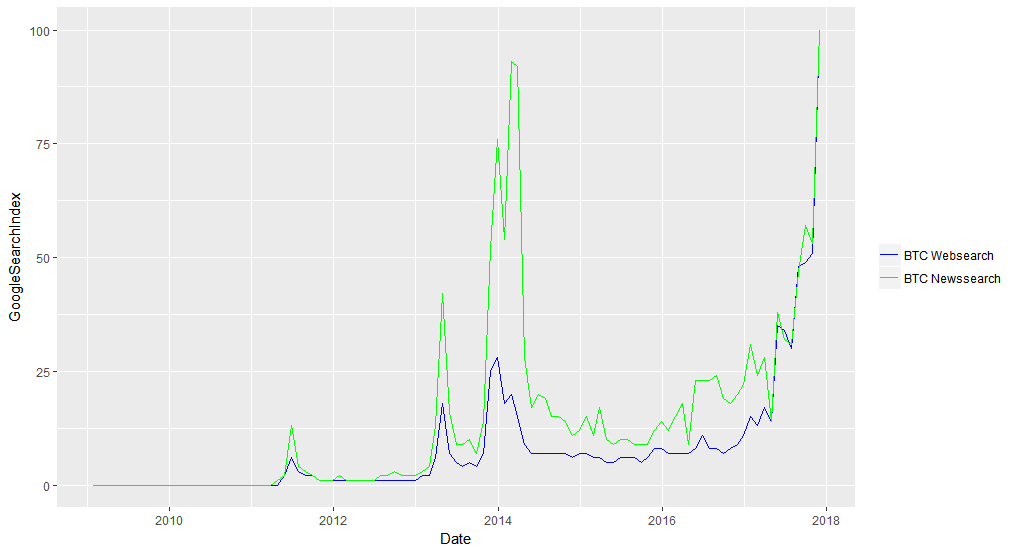
\includegraphics[width=\textwidth]{images/BTCpublicWithoutPrice}}
\caption{Google Websuchen und Newssuchen für "Bitcoin" im zeitlichen Verlauf}
\label{fig:PublicInterestBTC}
\centering
\end{figure}
Interpretiert man die Googlesuchen als Indikator für den Bekanntheitsgrad des Bitcoins, so lässt sich daraus schließen, dass die Währung bis 2011 sehr unbekannt und erst nach 2013 wirklich bekannt war. Zieht man nun den Bitcoinkurs heran (Listing \ref{list:PublicInterestBTC2}), so lässt sich ein Zusammenhang erkennen (Abbildung \ref{fig:PublicInterestBTC2}). 
\lstinputlisting[caption=Google Websuchen und Newssuchen für "Bitcoin" und Bitcoinkurs im zeitlichen Verlauf in R,label=list:PublicInterestBTC2]{../R/punlicInterestPlots/PublicInterestBTC2.R}
\begin{figure}[H]
\frame{
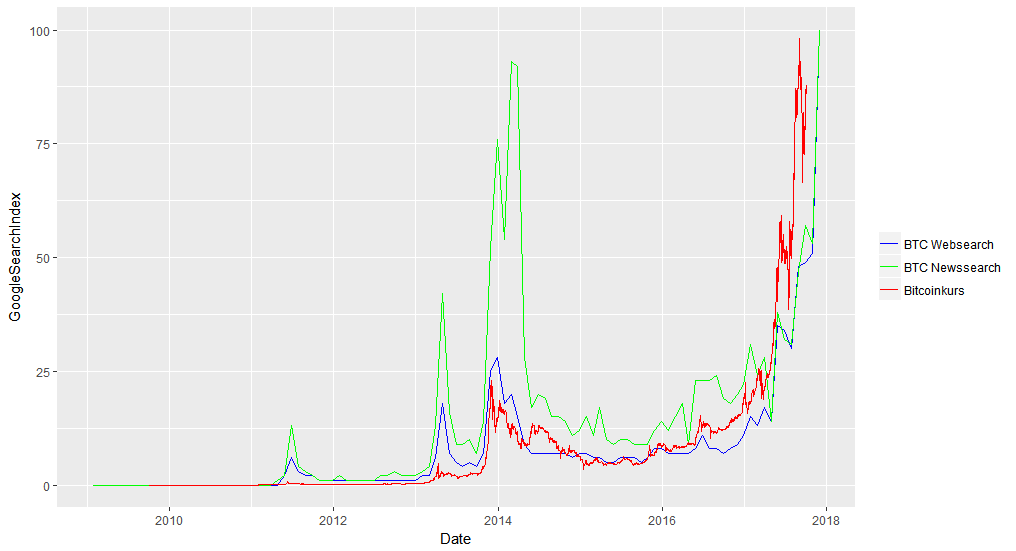
\includegraphics[width=\textwidth]{images/BTCpublicWithPrice}}
\caption{Google Websuchen und Newssuchen für "Bitcoin" im zeitlichen Verlauf}
\label{fig:PublicInterestBTC2}
\centering
\end{figure}
Anzumerken ist, dass die historischen Kursdaten hier in keinem Verhältnis zur y-Achse stehen und nur der grafischen Darstellung dienen.
Anders verhält es sich bei Etherum (siehe Abbildung \ref{fig:PublicInterestETH}). Hier besteht schon vor dem offiziellen Start des Etherumnetzwerks\citep{tual_ethereum_2015} ein gewisses Interesse.
\begin{figure}[H]
\frame{
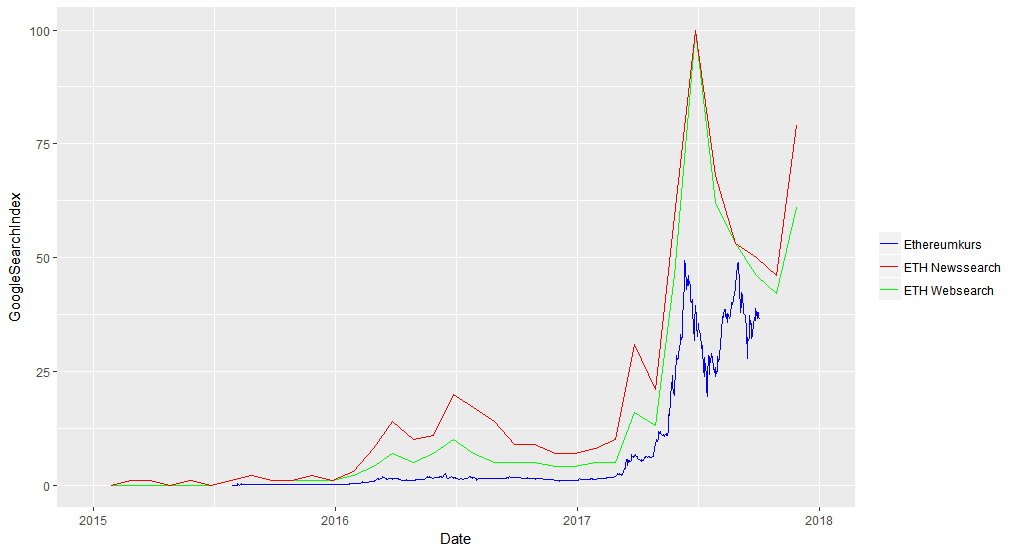
\includegraphics[width=\textwidth]{images/ETHpublicWithPrice}}
\caption{Google Websuchen und Newssuchen für "Ethereum" im zeitlichen Verlauf}
\label{fig:PublicInterestETH}
\centering
\end{figure}
Als Schlussfolgerung lässt sich daraus ableiten, dass es sehr unwahrscheinlich ist, dass Indikatoren wie Aktienindices oder der Ölpreis den Kryptowährungskurs beeinflussen, wenn sie noch unbekannt ist. Deswegen empfiehlt sich für die Analyse der Zeitraum, seit die Währungen Bekanntheit erlangt haben. 

\begin{longtable}[H]{|p{4,5cm}|p{12cm}|}
\hline
\textbf{Output} & \textbf{Beschreibung} \\ 
\hhline{==}
Data exploration report & Analyse des Bitcoinkurses erst ab 1.1.2011; des Etherumkurses ab 30.7.2015\\
\hline
\caption{Output des Schrittes "Explore the Data"}
\end{longtable}


\subsection{Verify Data Quality}
Bei der Sicherung der Datenqualität fällt auf, dass die Daten oberflächlich eine hohe Qualität aufweisen. Beispielsweise sind alle Datensätze in USD angegeben und strukturiert. Sie enthalten pro Datei nicht viele Features und besitzen kaum lückenhafte Spalten. Jedoch sind einige Dinge zu beachten (siehe Tabelle \ref{tab:dataQual}).

\begin{longtable}[H]{|p{5,5cm}|p{8,5cm}|}
\hline
\textbf{Problem} & \textbf{Lösung} \\ 
\hhline{==}
Die verschiedenen Datensätze haben unterschiedliche Datumsformate. Dies birgt Risiken beim Zusammenführen der Daten. & Vor dem Joinen der Daten müssten die Formate uniformiert werden. Dies kann beispielsweise mit der R-Methode \begin{lstlisting}
as.Date(data$DateColumn,format='%Y%m%d')
\end{lstlisting}
geschehen, solange das Datum in einem gültigen Format ist. \\ \hline
Beim Zusammensetzten der Datensätze entstehen Lücken, da einige Datensätze (z.B. Kryptowährungs-eigene Eigenschaften) sieben Observations pro Woche festhalten, Andere (z.B. Aktienindices) nur fünf. Außerdem gibt es Datensätze mit Feiertagen (z.B. Neujahr) oder solche mit nur einer Observaton pro Woche (z.B. STLFSI). & Azure ML Studio bietet das Experiment Item 'Clean Missing Data' an. Neben den Möglichkeiten, fehlende Daten mit dem Modus, Median oder Mittelwert auszufüllen, kann das Verfahren MICE\citep{azur_multiple_2011} oder die Probablilistic PCA\citep{tipping_probabilistic_1999} genutzt werden. \\ \hline
Durch die unterschiedlichen Formatierungen gibt es inkonsistente Separatoren (Komma, Semikolon, Tab), Dezimaltrennzeichen (Punkt, Komma) und Tausendertrennzeichen (Punkte, ohne Trennzeichen). & Vor dem Zusammenführen müssen die Separatoren und Trennzeichen untersucht und eventuell umgeändert werden. Dies kann mit Excel ('Speichern als...' oder Notepad++ ('Find and Replace') geschehen. Nach dem Joinen muss nachgeprüft werden. \\ \hline
Die Schwierigkeit für das Etherumining wird im Datensatz ethereumDataset anfangs mit kleiner als 1 angeben. Dies ist per Definition unmöglich. & Entweder es handelt sich hier um einen undokumentierte Sonderfall zu Beginn des Netztwerks oder es ist ein Fehler im Datensatz. Trotz dieser Unstimmigkeit, ist die Tatsache insignifikant und kann vernachlässigt werden. \\ \hline
\caption{Data quality report des Schrittes "Verify data quality"}
\label{tab:dataQual}
\end{longtable}

hier aufzählen alles und bei select dann reduzieren und bei clean dann lücken etc.
bei construict dann bis zu azure zusammenbauen 


\section{Data Preperation}
\subsection{Select Data}
Die Datensätze sind nun gut beschrieben und es wurde auf Herausforderungen und Probleme hingewiesen. Die folgenden Punkte befassen sich damit, die richtigen Daten und Features weiter zu reduzieren ("Select Data"), sie zu reinigen ("Clean Data") und schließlich zum endgültigen Analyse-Datensatz zusammenfassen ("Construct Data", "Integrate Data" und "Format Data").
Ausgenommen der jetzt begründet ausgeschlossenen Daten, werden alle Vorgestellten zum bilden des Models genutzt. Tabelle \ref{tab:selecData} liefert einen Überblick.

In Punkt \ref{subsec:collection} wurde festgestellt, dass der Datensatz 'BTC \textunderscore Total \textunderscore Volume \textunderscore Daily \textunderscore Full' große Lücken enthält. Darüber hinaus enthält der Datensatz 'bitcoinDataset' ebenfalls die Anzahl der Bitcoins als Feature 'btc \textunderscore total \textunderscore bitcoins'. Ein stichprobenhafter Konsistenzcheck ergibt, dass die vorhanden Daten sich decken. Aus diesem Grund wird der Lückenhafte Datensatz exkludiert. 
'BTC \textunderscore Difficulty \textunderscore Daily \textunderscore Full' enthält wie 'bitcoinDataset' die Miningschwierigkeit (siehe Punkt \ref{sec:cryptocurrency2}). Obwohl der einzelne Datensatz minimal genauere Werte enthält, fällt die Wahl erneut auf das 'bitcoinDataset', da es Daten über eine längere Zeitspanne enthält. Genauso verhält sich bei 'BTC \textunderscore Transaction \textunderscore Number \textunderscore Fully \textunderscore Daily' und 'BTC \textunderscore Price \textunderscore Multiple \textunderscore Daily'. 
Analog wird bei den Etherumdatensätzen vorgegangen. 'ETH \textunderscore Total \textunderscore Volume \textunderscore Daily \textunderscore Full' enthählt die gleichen Daten wie 'ethereumDataset'. Allerdings um Faktor 100000 erhöht. Vermutlich handelt es sich hierbei um eienn Konvertierungs- oder Kopierfehler, da das derzeit mögliche Maximum bei 100 Millionen Ether liegt.\multicitep{buterin_lets_2016; hawksby-robinson_what_2017} Die Werte für die Schwierigkeit und Anzahl der Transaktionen stimmen bei 'ETH \textunderscore Difficuly \textunderscore Daily \textunderscore Full' bzw. 'ETH \textunderscore Transaction \textunderscore Number \textunderscore Fully' mit 'ethereumDataset' genau überein. 
Auch wenn die Datensätze an dieser Stelle aussortiert werden, war ihre Beschreibung keine Verschwendung. Sie hat dazu beigetragen, das Domainwissen (siehe \ref{} \todo{anfügen}) zu vertiefen und die Plausibilität der Daten zu prüfen.


\begin{longtable}[H]{|p{11cm}|p{2,5cm}|p{2,5cm}|}
\hline
\textbf{Datensatz} & \textbf{Inkludiert} & \textbf{Exkludiert} \\ 
\hhline{===}
BTC \textunderscore Total \textunderscore Volume \textunderscore Daily \textunderscore Full & & X \\ \hline
BTC \textunderscore Difficulty \textunderscore Daily \textunderscore Full & & X \\ \hline
BTC \textunderscore Transaction \textunderscore Number \textunderscore Fully \textunderscore Daily & & X \\ \hline
BTC \textunderscore Price \textunderscore Multiple \textunderscore Daily & & X \\ \hline
ETH \textunderscore Total \textunderscore Volume \textunderscore Daily \textunderscore Full & & X \\ \hline
ETH \textunderscore Difficuly \textunderscore Daily \textunderscore Full & & X \\ \hline
ETH \textunderscore Transaction \textunderscore Number \textunderscore Fully \textunderscore Daily & & X \\ \hline
google \textunderscore Trends \textunderscore BTC \textunderscore Websearch &  & \\ \hline
google \textunderscore Trends \textunderscore ETH \textunderscore Websearch &  & \\ \hline
google \textunderscore Trends \textunderscore BTC \textunderscore Newssearch &  & \\ \hline
google \textunderscore Trends \textunderscore ETH \textunderscore Newssearch &  & \\ \hline
Wiki \textunderscore Page \textunderscore Views \textunderscore BTC & & \\ \hline
Wiki \textunderscore Page \textunderscore Views \textunderscore ETH &  & \\ \hline
abcnews \textunderscore Date \textunderscore  & & \\ \hline
\caption{Inkludierte und exkludierte Datensätze für die Analyse}
\label{tab:selecData}
\end{longtable}

-aktienindices: nicht alle brauchen, weil sonst überrepresantiv; für btc nur die ab 1.1.2011; nicht zwei getrennte, deswegen auf diesen für ETH nutzen
-change\%: oft angesprochen, jetzt gekillt, kein mehrwert nur für menschen besser lesbar, reduzieren gut für algorithmen, jetzt nicht mitnehmen. das ist der fall bei aktienidices, währungen und natürliche ressourcen

-textding oh fuck




\subsection{Clean Data}
Ziel: Sachen aus "Verfiy Data Quality" aufgreifen;
--> Lücken füllen, Preise, Datum

evtl. was könnte noch ein problem werden?

\subsection{Construct Data}
Ziel: Daten so umbauen, dass sie in algorithmus passen
umfasst evtl. abgeleitete attribute; hier aber nicht. eig schon, da indices v.a stfl sehr starkt zusammenfassende dinge sind

--> aggregieren in super-datensätze für katheogien wegen azure
output: aggregierte, saubere daten


\subsection{Integrate Data}
Ziel: Daten zusammenführen
--> die fertigen Datensätze, die ich gefunden habe in die BTC-, ETH-Kursdaten überführen
--> in azure machen mit join

\subsection{Format Data}
mal sehen, ob es auch so geht; evtl. namen der sachen ändern, damit die sachen nicht gleich heißen! (vorgreifen in construct/integrate)






\section{Modeling}
\subsection{Select the Modeling Technique}
Ziel: Auswahl der Algorithmen
--> Supervised (Continous value --> wert; two-class (hoch/runter))

\subsection{Generate Test Design}
Ziel: Training und error rates betrachten
--> azure split data experiment item!

\subsection{Build the Model}
Ziel: Models bauen
--> "azure ml run"

\subsection{Assess the Model}


\section{Evaluation}
\subsection{Evaluate Results}
\subsection{Review Process}
\subsection{Determine Next Steps}


\section{Deployment}
\subsection{Plan Deployment}
\subsection{Plan Monitoring and Maintenance}
\subsection{Produce Final Report}
\subsection{Review Project}


